\documentclass[spanish,12pt]{article}
\usepackage[spanish]{babel}
\usepackage[utf8]{inputenc}
\usepackage{xspace}
\usepackage{lmodern}
\usepackage{indentfirst}
\usepackage{xargs}
\usepackage{ifthen}
\usepackage{fancyhdr}
\usepackage{latexsym}
\usepackage{lastpage}
\usepackage{textcomp}
\usepackage{varwidth}
\usepackage{caratula, aed2-tad,aed2-symb,aed2-itef}
\usepackage{algorithmicx, algpseudocode, algorithm}
\usepackage{enumerate}
\usepackage{graphicx}
\usepackage{caption}
\usepackage{subcaption}
\usepackage{float}
\usepackage{anysize}
\marginsize{1.5cm}{1.5cm}{1.5cm}{1.5cm}

\begin{document}

\titulo{Informe 1}
\materia{Algoritmos y Estructuras de Datos III}
\author{Grupo  \\Alvarez Vico Jazm\'in\\Cortés Conde Titó Javier María\\Pedraza Marcelo \\ Rozenberg Uriel Jonathan}

\integrante {Jazmín Alvazer Vico}{75/15}{jazminalvarezvico@gmail.com}
\integrante {Marcelo Pedraza}{393/14}{marcelopedraza314@gmail.com}
\integrante {Uriel Jonathan Rozenberg}{838/12}{rozenberguriel@gmail.com}
\integrante {Javier María Cortés Conde Titó}{252/15}{javiercortescondetito@gmail.com}

\maketitle


\clearpage

\tableofcontents
\cleardoublepage

\section{Problema 1: Cruzando el puente}

\subsection{Inrtoducción}

En este problema, un grupo formado por arquéologos y caníbales debe cruzar un puente. El mismo sólo puede ser atravezado por dos personas a la vez, y tiene que ser cruzado con una linterna. Como el grupo sólo dispone de una linterna, siempre debe regresar alguno al lado del puente original. Además, en ningún lado del puente puede haber más caníbales que arquéologos.
Cada individuo consta de la propiedad "velocidad", un número natural que indica cuánto tiempo tarda en atravezar el puente. Si dos personas atraviezan el puente juntas, lo hacen en el tiempo más grande entre los dos.

%terminar%

\subsection{Explicación de la solución}

%%%%%%%%%%%%%%%%%%%%%%%%%%%%%%%%%%%%%%%%%%%%%%%%%%%

\section{Problema 2: Problemas en el camino}

\subsection{Introducción}

En el problema enunciado, Nuestros exploradores se encuentran con una balanza de dos platos, y en el de la izquierda la llave que necesitan. Para que esta sea de utilidad, al tomarla deben mantener la posición de la balanza y para realizar esto cuentan con pesas de peso igual a las potencias de tres (una pesa por potencia).
Entonces, sabiendo el peso de la llave, necesitamos saber que pesas poner en cada plato para mantener el equilibrio original.
Podemos pensar que el lado derecho de la balanza equivale a la operación de sustracción y el izquiero a la adición. De esta forma al agregar pesas de un lado o del otro estariamos sumando o restando su peso.
Formalmente esto equivale a decir que, si tenemos un entero n queremos sumar o restar potencias de tres, sin repetirlas hasta alcanzar su valor.

\subsection{Explicación de la solución}

Para resolver este problema, Reescribimos P en la base ternaria, es decir, a este valor los notaremos T. Entonces tenemos $P = \sum_{i=0}^{n} a_i3^i$  con $0 \leq a_i \leq 2$ y $n = log_{3}{(P)}$  entonces $T ={a_1,a_2,...,a_n}$.
Luego, se toman en orden uno a uno los elementos de T. si $a_i$ es 0, no hacemos nada. Si $a_i$ es 1, en la balanza izquierda ponemos la pesa que corresponde a $3^i$. si $a_i =2$, ponemos una pesa de $3^i$ en la balanza derecha y sumamos 1 a $a_{(i+1)}$ (y consecuentemente, se cambian los valores posteriores de T para que sigan en base ternaria)


\subsubsection{Pseudocódigo}

Nota: Para la implementación, en vez de crear el conjunto T, vamos tomando el resto de P y diviendolo por 3 entonces, el valor de la variable "rem" sería el equivalente al $a_i$ (i responde al numero de iteraciones ya hechas)

\begin{algorithm}[H]{\textbf{Pesas}(Natural: P)}
	\begin{algorithmic}[1]
		\State pesa $\gets$ 1
		\While{ P $>$ 0}
		 	\State rem $\gets$ $r_3 (P)$
	    		\State P $\gets $ parte entera(P/3)
	    		\If{rem = 1}
	    			\State pesa va para la balanza izquierda    			\Else
				\If{ rem = 2}
	    				\State p$\gets$ P+1
	    				\State pesa va para la balanza derecha
				\EndIf
			\EndIf
			\State pesa $\gets$ pesa*3
		\endWhile
	\end{algorithmic}
\end{algorithm}



\subsubsection{Demostración de Correctitud}

Primero probaremos un lema inductivamente: 
$\forall n \in N$ vale que  $2*3^{n} = 3^{n+1}-3^{n}$.

Caso base: 
queremos ver que $2*3^{0} = 3^{1}-3^{0}$
$2*3^0 = 2*1=2$ y $3^1-3^0= 3-1=2$ entonces $2*3^{0} = 3^{1}-3^{0}$
\\
\\
Hipótesis Inductiva: 
$\forall n \in N$ vale que  $2*3^{n} = 3^{n+1}-3^{n}$
\\
\\
Paso Inductivo: 
queremos ver que $\forall n \in N$ vale que  $2*3^{n+1} = 3^{n+2}-3^{n+1}$

$2*3^{n+1} = 2*3^{n}*3 $
\\
 por hipotesis inductiva: $2*3^{n}*3 = (3^{n+1}-3^{n})*3 = 3^{n+1}*3 - 3^{n}*3= 3^{n+2}-3^{n+1} $
\\
luego, como valen el caso base y el paso inductivo, entonces vale $2*3^{n} = 3^{n+1}-3^{n} \forall n \in N $ 

\\
Ahora para probar la correctitud del algoritmo, desarrollaremos algunos conceptos algebraicos.
Por el algoritmo de división de Euclides sabemos que podemos escribir \\  $P= q*3+ r_{3}(P)$ con $0\leq r_{3}(P) \leq 2 $ luego, podemos escribir $q= z*3 + r_{3}(q)$ entonces $P= (z*3 + r_{3}(q))*3 +r_{3}(P)$ y así recursivamente y aplicando la distributividad de la suma podemos descomponer p en las potencias de 3. finalmente obtendriamos $p= \sum_{i=0}^{n}{a_i 3^{i}} $ con $0 \leq a_i \leq 2$.
Ahora nuestro problema es la aparición de $a_i=2$ en la descomposición puesto que solo tenemos una pesa por potencia de tres. Pero por lo visto en el lema anterior, $2*3^{i}= 3^{i+1}-3^{i}$ esto equivale a poner la pesa $3^{i+1}$ en la balaza izquierda y la $3^{i}$ en la derecha obteniendo el equivalente a 2 pesas $3^{1}$ en la izquierda. aplicando este proceso recursivamente, obtenemos  una descomposición de P sumando y restando sus potencias de tres sin repeticiones. 


\subsubsection{Demostración de Complejidad}

El algoritmo consta de un ciclo, dentro de cada iteración, se calcula el resto y hace dos comparaciones todas estas operaciones se ejecutan en O(1), mientras que enviar la pesa a cada balanza
es agregar un número al final de una lista, ya que el modelo de lista que usamos es "METERMODELO", esto se realiza en O(1).
Entonces, dentro de cada iteración solo se hacen operaciones en O(1). Esto hace que la complejidad sea la cantidad de iteraciones que hace el ciclo.

Si nos abstraemos del if, el ciclo tiene como condición que P>0, siendo P el valor de entrada. Como podemos observar P es modificado dividiendose por 3 por cada iteración. Por algebra básica sabemos que se necesesitaran como mucho log_3(P) + 1 iteraciones para q P sea menor a 0.
Ahora, tomando en cuenta el if hay un caso en el cual le sumamos 1 a P, lo cual afecta un poco la cuenta, si volvemos a la explicacion del algoritmo y tomamos el conjunto T = {a_1,...,a_n}
donde  $P = \sum_{i=0}^{n} a_i3^i$  con $0 \leq a_i \leq 2$ y $n = log_{3}{P}$, siendo el valor de rem el valor de a_i en la iesima iteracion.
Cuando hacemos que P<- P+1 nos queda que en la proxima iteracion rem valdria uno mas, es decir a_(i+1) pasaria a valer uno mas de lo q valdria en T. Ahora,  siendo estos que para todo a_k
valen entre 0 y 2, si a_(i+1) en vez de valer 3, valdria 0 y a_(i+2) valdria uno mas tambien, y si  a_(i+2) valia 2, pasaria a valer 0 y  a_(i+3) valdria uno mas y asi sucesivamente hasta llegar a a_n.
y si resulta que tambien a_n valia 2, entonces tendriamos un a_(n+1) que entraria a valer 1 y a_n valdria 0.
Luego no habria mas casos donde a_j (para i<j<=n) donde a_j sea 2, entonces no hay mas casos donde puedan volver a ocurrir este tipo de cosas, quedandonos asi, un maximo de Log_3(P)+1 iteraciones

Entonces, la complejidad del algoritmo es de $\mathcal{O}(Log_{3}(P))$.
Luego, se puede probar que Log(P) es $\mathcal{O}(\sqrt(P))$


\subsection{Experimentación}

\subsubsection{Resultados}

\subsubsection{Análisis}




%%%%%%%%%%%%%%%%%%%%%%%%%%%%%%%%%%%%%%%%%%%%%%%%%%%%%%%%%%%%%%%%%%%%%%%%%%%%%%%%%%%%%%%%%%%%%

\section{Problema 3: Guardando el tesoro}

\subsection{Introducción}

En este problema, los exploradores se encuentran frente a muchos tesoros que desearían poder llevarse. Para esto, cuentan con varias mochilas, cada una con una determinada capacidad de peso que puede cargar.
Los tesoros son de distintos tipos, y cada tipo tiene un peso y un valor determinado.
El objetivo es encontrar la manera optima de llenar las mochilas para poder llevar el mayor valor posibe.

Formalmente, tenemos un conjunto de elementos que tienen como propiedad dos naturales asociados (el peso y el valor). Entonces podemos inferir que existen dos criterios de ordenamiento asociados respectivamente a estos valores.
Al mismo tiempo tenemos otro conjunto de elementos que posee como propiedad un natural asociado (capacidad).
Nuestro objetivo es seleccionar una combinación de los primeros objetos, restringida por las capacidades dadas,de modo de maximizar la sumatoria del valor de los mismos.


\subsection{Explicación de la solución}

   Inicialmente creimos que este problema podría resolverme mediante un algoritmo de BackTracking, sin embargo observamos que nunca lograríamos conseguir la complejidad pedida puesto que este tipo de algoritmos conlleva una complejidad exponencial sperior a la pedida.
   Finalmente pudimos resolverlo mediante prmathcal{O}amación dinámica. Nuestro algoritmo principal llama a dos funciones que utilizan la recursividad para podes obtener en un caso el valor óptimo, y en el otro "las mochilas llenas."
   Para facilitar el entendimiento del algoritmo introduciremos el concepto de "Hipercubo". Un hipercubo es el analogo n-dimensional de un cuadrado (n=2) o un cubo (n=3). En particular en nuestro problema tenemos un hipercubo de dimension cuatro, estaa figura se denomina "teseracto" sin embargo por comodidad seguiremos llamandole hipercubo en el resto del informe. 
Para poder imaginar este concepto, podriamos visualizarlo en nuestro mundo tridimencional como un vector con cubos adentro. la cantidad de cubos dependera del largo de nustro cuarta "arista".

%dibujito%

observación: nuestro algoritmo descarta los tesoros que tienen un peso mayor al maximo de capacidad entre las mochilas. Asumimos en el pseusocodigo que nuestra entrada cumple esa propiedad.


\subsubsection{Pseudocódigo}

\begin{algorithm}[H]{\textbf{guardandoTesoro}(mochilas: vector$<$mochila$>$, cofre: vector$<$tesoro$>$)}
	\begin{algorithmic}[1]
		\State objXpesos $\gets$ Hipercubo() incializado en -1 \Comment (en las posiciones donde no puede haber objetos incializo en 0) $\mathcal{O}$()
		\State sol= ValorOptimo(objXpesos,cofre,cofre.size-1,capacidades de las mochilas)
		\State LlenarMochilas(objXpesos, cofre, mochila1, mochila2, mochila3)
		\State return (sol, mochilas)
	\end{algorithmic}
\end{algorithm}



\begin{algorithm}[H]{\textbf{LlenarMochilas}(objetoXpeso: hipercubo, cofre:vector$<$tesoro$>$, m1,m2,m3:mochilas)}
	\begin{algorithmic}[1]
		\State desde i= cofre.size-1 hasta i=0
			\State obj $\gets$ cofre[i]
			\State cap1 $\gets$ m1.Capacidad
			\State cap2 $\gets$ m2.Capacidad
			\State cap3 $\gets$ m3.Capacidad
			\If{$i=0$}
				\State Agregar obj en cualquier mochila en la que entre.
			\Else
				\State valM1 $\gets$ obj.valor + ValorOptimo(objetoXPeso, cofre, i,cap1-obj.peso,cap2,cap3 )
				\State valM2 $\gets$ obj.valor + ValorOptimo(objetoXPeso, cofre,i,cap1,cap2-obj.peso,cap3 )
				\State valM3 $\gets$ obj.valor + ValorOptimo(objetoXPeso, cofre,i, cap1, cap2,cap3-obj.peso )	
				\State MeterEnCorrecta(valM1,valM2,valM3,m1,m2,m3,obj)
			\EndIf

	\end{algorithmic}
\end{algorithm}



%%%

\begin{algorithm}[H]{\textbf{ValorOptimo(objXpeso:hipercubo, cofre:vector$<$tesoro$>$, objeto:int, peso1: int, peso2:int, peso3:int)}}
	\begin{algorithmic}[1]
		\State  pesoObj $\gets$ cofre[objeto].peso \Comment $\mathcal{O}$(1)
		\State  pesoVal $\gets$ cofre[objeto].valor \Comment $\mathcal{O}$(1)

		\If{$peso1 < 0 \vee peso2 < 0 \vee peso3 < 0$}
			\State return $-1$ \Comment \mathcal{O}(1)

		\EndIf

		\If{objetoxPesos[objeto][peso1][peso2][peso3] $\neq$ -1}
			\State return objetoxPesos[objeto][peso1][peso2][peso3] \Comment $\mathcal{O}$(1)
		\EndIf
		\If{objeto $=$ 0}
			\State val $\gets$ 0 \Comment \mathcal{O}(1)
			\If{peso1 $\ge$ pesoObj $\vee$ peso2 $\ge$ pesoObj $\vee$ peso3 $\ge$ pesoObj}
				\State val $\gets$ valorObj \Comment \mathcal{O}(1)
				\State objetoxPesos[objeto][peso1][peso2][peso3] $\gets$ val \Comment $\mathcal{O}$(1)
				\State return val \Comment $\mathcal{O}$(1)
			\EndIf

		\Else
			\State PosiblesSolus $\gets$ vector$<$int$>$ \Comment $\mathcal{O}$(1)
			\State sinObj $\gets$ ValorOptimo(objetoxPesos, cofre, objeto -1, peso1, peso2, peso3)
			\State PosiblesSolus.Agregar(sinObj)
			\If{peso1-pesoObj $\ge$ 0}
				\State objen1 $=$ valorObj + ValorOptimo(objetoxPesos, cofre, objeto - 1, peso1 - pesoObj, peso2, peso3)
				\State PosiblesSolus.Agrergar(objen1)
			\EndIf
			\If{peso2 - pesoObj $\ge$ 0}
				\State objen2 = valorObj + ValorOptimo(objetoxPesos, cofre, objeto - 1, peso1, peso2  - pesoObj, peso3)
				\State PosiblesSolus.Agregar(objen2)
			\EndIf
			\If{peso3-pesoObj $\ge$ 0}
				\State objen3 = valorObj + ValorOptimo(objetoxPesos, cofre, objeto - 1, peso1, peso2, peso3  - pesoObj)
				\State PosiblesSolus.Agregar(objen3)
			\EndIf
			\State valor=Max(PsiblesSolus)
			\State objetoxPesos[objeto][peso1][peso2][peso3] = valor
			\State return valor
		\EndIf


	\end{algorithmic}
\end{algorithm}

\newpage

\subsubsection{Demostración de Correctitud}
Presentaremos la función matemática que modela nuestro problema:\\

$f(o,p_{1},p_{2},p_{3})=0 \\
f(n,p_{1},p_{2},p_{3}) = Max(V_{n}+Max(f(n-1,p_{1}-p_{n},p_{2},p_{3}), f(n-1,p_{1},p_{2}-p_{n},p_{3}), f(n-1,p_{1},p_{2},p_{3}-p_{n})),f(n-1,p_{1},p_{2},p_{3})) $
\\
Donde n representa el numero de tesoro, $V_{n}$ y $P_{n}$ su valor y su peso respectivamente. $p_{1},p_{2}\ y \ p_{3}$ son las capacidades de cada mochila.

Para la demostración utilizaremos inducción global en n.
\\
\\
Caso base: queremos ver que $f(0,p_{1},p_{2},p_{3})$ resulta ser el valor máximo que se puede obtener con 0 objetos:
$f(0,p_{1},p_{2},p_{3}) = 0$ al tener 0 objetos el valor de los mismos es 0 de modo que es el máximo valos posible.
\\
\\
Hipotesis Inductiva: $\forall k<n$ vale que $f(k,p_{1},p_{2},p_{3})$ da el valor máximo que se puede obtener con k objetos.
\\
\\
Ahora queremos ver que $f(n,p_{1},p_{2},p_{3})$ da el valor óptimo para n objetos.
\\
\\
$f(n,p_{1},p_{2},p_{3}) = Max(V_{n}+Max(f(n-1,p_{1}-p_{n},p_{2},p_{3}), f(n-1,p_{1},p_{2}-p_{n},p_{3}), f(n-1,p_{1},p_{2},p_{3}-p_{n})),f(n-1,p_{1},p_{2},p_{3})) $ \\
por hipótesis inductiva (como $n-1 \leq k$ para algun k) sabemos que $f(n-1,p_{1}-p_{n},p_{2},p_{3}), f(n-1,p_{1},p_{2}-p_{n},p_{3}), f(n-1,p_{1},p_{2},p_{3}-p_{n}) y f(n-1,p_{1},p_{2},p_{3})$ son los valores optimos que se pueden conseguir con n-1 objetos restando (o no) el peso del objeto n de modo de luego poder guardarlo en alguna mochila (o no). utilizaremos los renombres $V_{01},V_{02},V_{03},V_{00}$ respectivamente.
Entonces tenemos: \\
$f(n,p_{1},p_{2},p_{3})= Max(V_{n}+Max(V_{01},V_{0,2},V_{03}),V_{00})$\\
Podemos ver que esta función  compara el valor optimo de llenar las mochilas con n-1 tesoros y el tesoro n, con el valor optimo de llenar las mochilas con n-1 tesoros sin el tesoro n (de esta forma se tiene cuenta el caso en el que el mejor valor se obtuviene de poner algun objeto  de los n-1 anteriores que impide luego meter el tesoro n).\\
Como la función Max devuelve el mayor valor, el resultado sera el óptimo.
\\
Como valen P(0)..p(k) $\forall k<n$ y vale p(n) $\Rigtharrow$ vale p(n) $\forall n \in N \cup {0} $

\subsubsection{Demostración de Complejidad}

Como se observa en el inciso () la complejidad del algoritmo GuardarTesoro es $\mathcal{O}(\prod_{i=1}^{3}K_{i} * T)$ donde $K_i$ representa la capacidad de cada mochila y T la cantidad de tesoros. Ademas esta complejidad es aportada por el algoritmo ValorOptimo, entonces basaremos nuestra demosrtación en el mismo.

Primero haremo unas observaciones preliminares:
\begin{itemize}

	\item El volumen de un cubo es es $\prod_{i=1}^{3}A_{i}$ donde cada $A_i$ es una arista que representa el eje de la altura, el ancho o el largo. Como explicamos en la introducción gracias a nuestro modelado, sabemos que llenar una posición del cubo nos cuesta $\Theta(1)$ entonces llenarlo entero nos costará el equivalente al volumen del mismo. Podriamos visualizarlo como subdividir un cubo en cubos pequeños de dimension 1X1X1.
	\item Llenar un hipercubo con un valor determinado (como ocurre en la linea 1 de guardandoTesoro) cuesta $\mathcal{O}(\prod_{i=1}^{3}K_{i} * T)$ ya que hay T cubos para llenar.
	\item Cuando se llama a LlenarMochilas desde GuardarTesoro cuesta $\mathcal{O}(T)$ ya que en en las lineas 9,10,11 cuando se llama a ValorOptimo, el hipercubo objetoXpeso cuenta con todos lo valores ya calculados entrando en el if (linea 6) que devuelve en $\mathcal{O}(1)$ el valor.
\end{itemize}

Volviendo a la demostración, tanto en el pseudocódigo como en la función matemática podemos ver que la recursión se realiza tantas veces como la cantidad total de tesoros. Para llenar un cubo, siempre debemos recurrir al cubo anterior, uno puede pensar que esto aportaría complejidad, sin embargo, al guardar estos valores solo construimos estos cubos una vez, y la complejidad por acceso es $\Theta(1)$.

Otra manera de verlo, es analoga a la explicacion de la complejidad de llenar un cubo. Al estar llenando un hipercubo la complejidad sera quivalente al hipervolumen del mismo, es decir, multiplicariamos las tres aristas anteriores por una que sería la cuarta dimensión(en este caso los tesoros).

De cualquier manera podemos concluir que la complejidad es $\mathcal{O}(\prod_{i=1}^{3}K_{i} * T)$

Ahora probemos que esta complejidad es menor a la pedida ($\mathcal{O}((\sum_{i=1}^{3}K_{i})^{3} * T)$)

$\prod_{i=1}^{3}K_{i}  = K_1*K_2*K_3$   sea $K_max = Max(K_1,K_2,K_3)$ y $K_o= K_1^3 + K_2^3 + K_3^3 - K_max^3$ entonces $K_1*K_2*K_3 < K_m^3 < K_m^3 + K_o = K_1^3+K_2^3+K_3^3 <(\sum_{i=1}^{3}K_{i})^{3}$ entonces $\prod_{i=1}^{3}K_{i}* T < \sum_{i=1}^{3}K_{i})^{3} * T $


\subsection{Experimentación}

\subsubsection{Resultados}

\begin{figure}[H]
\centering
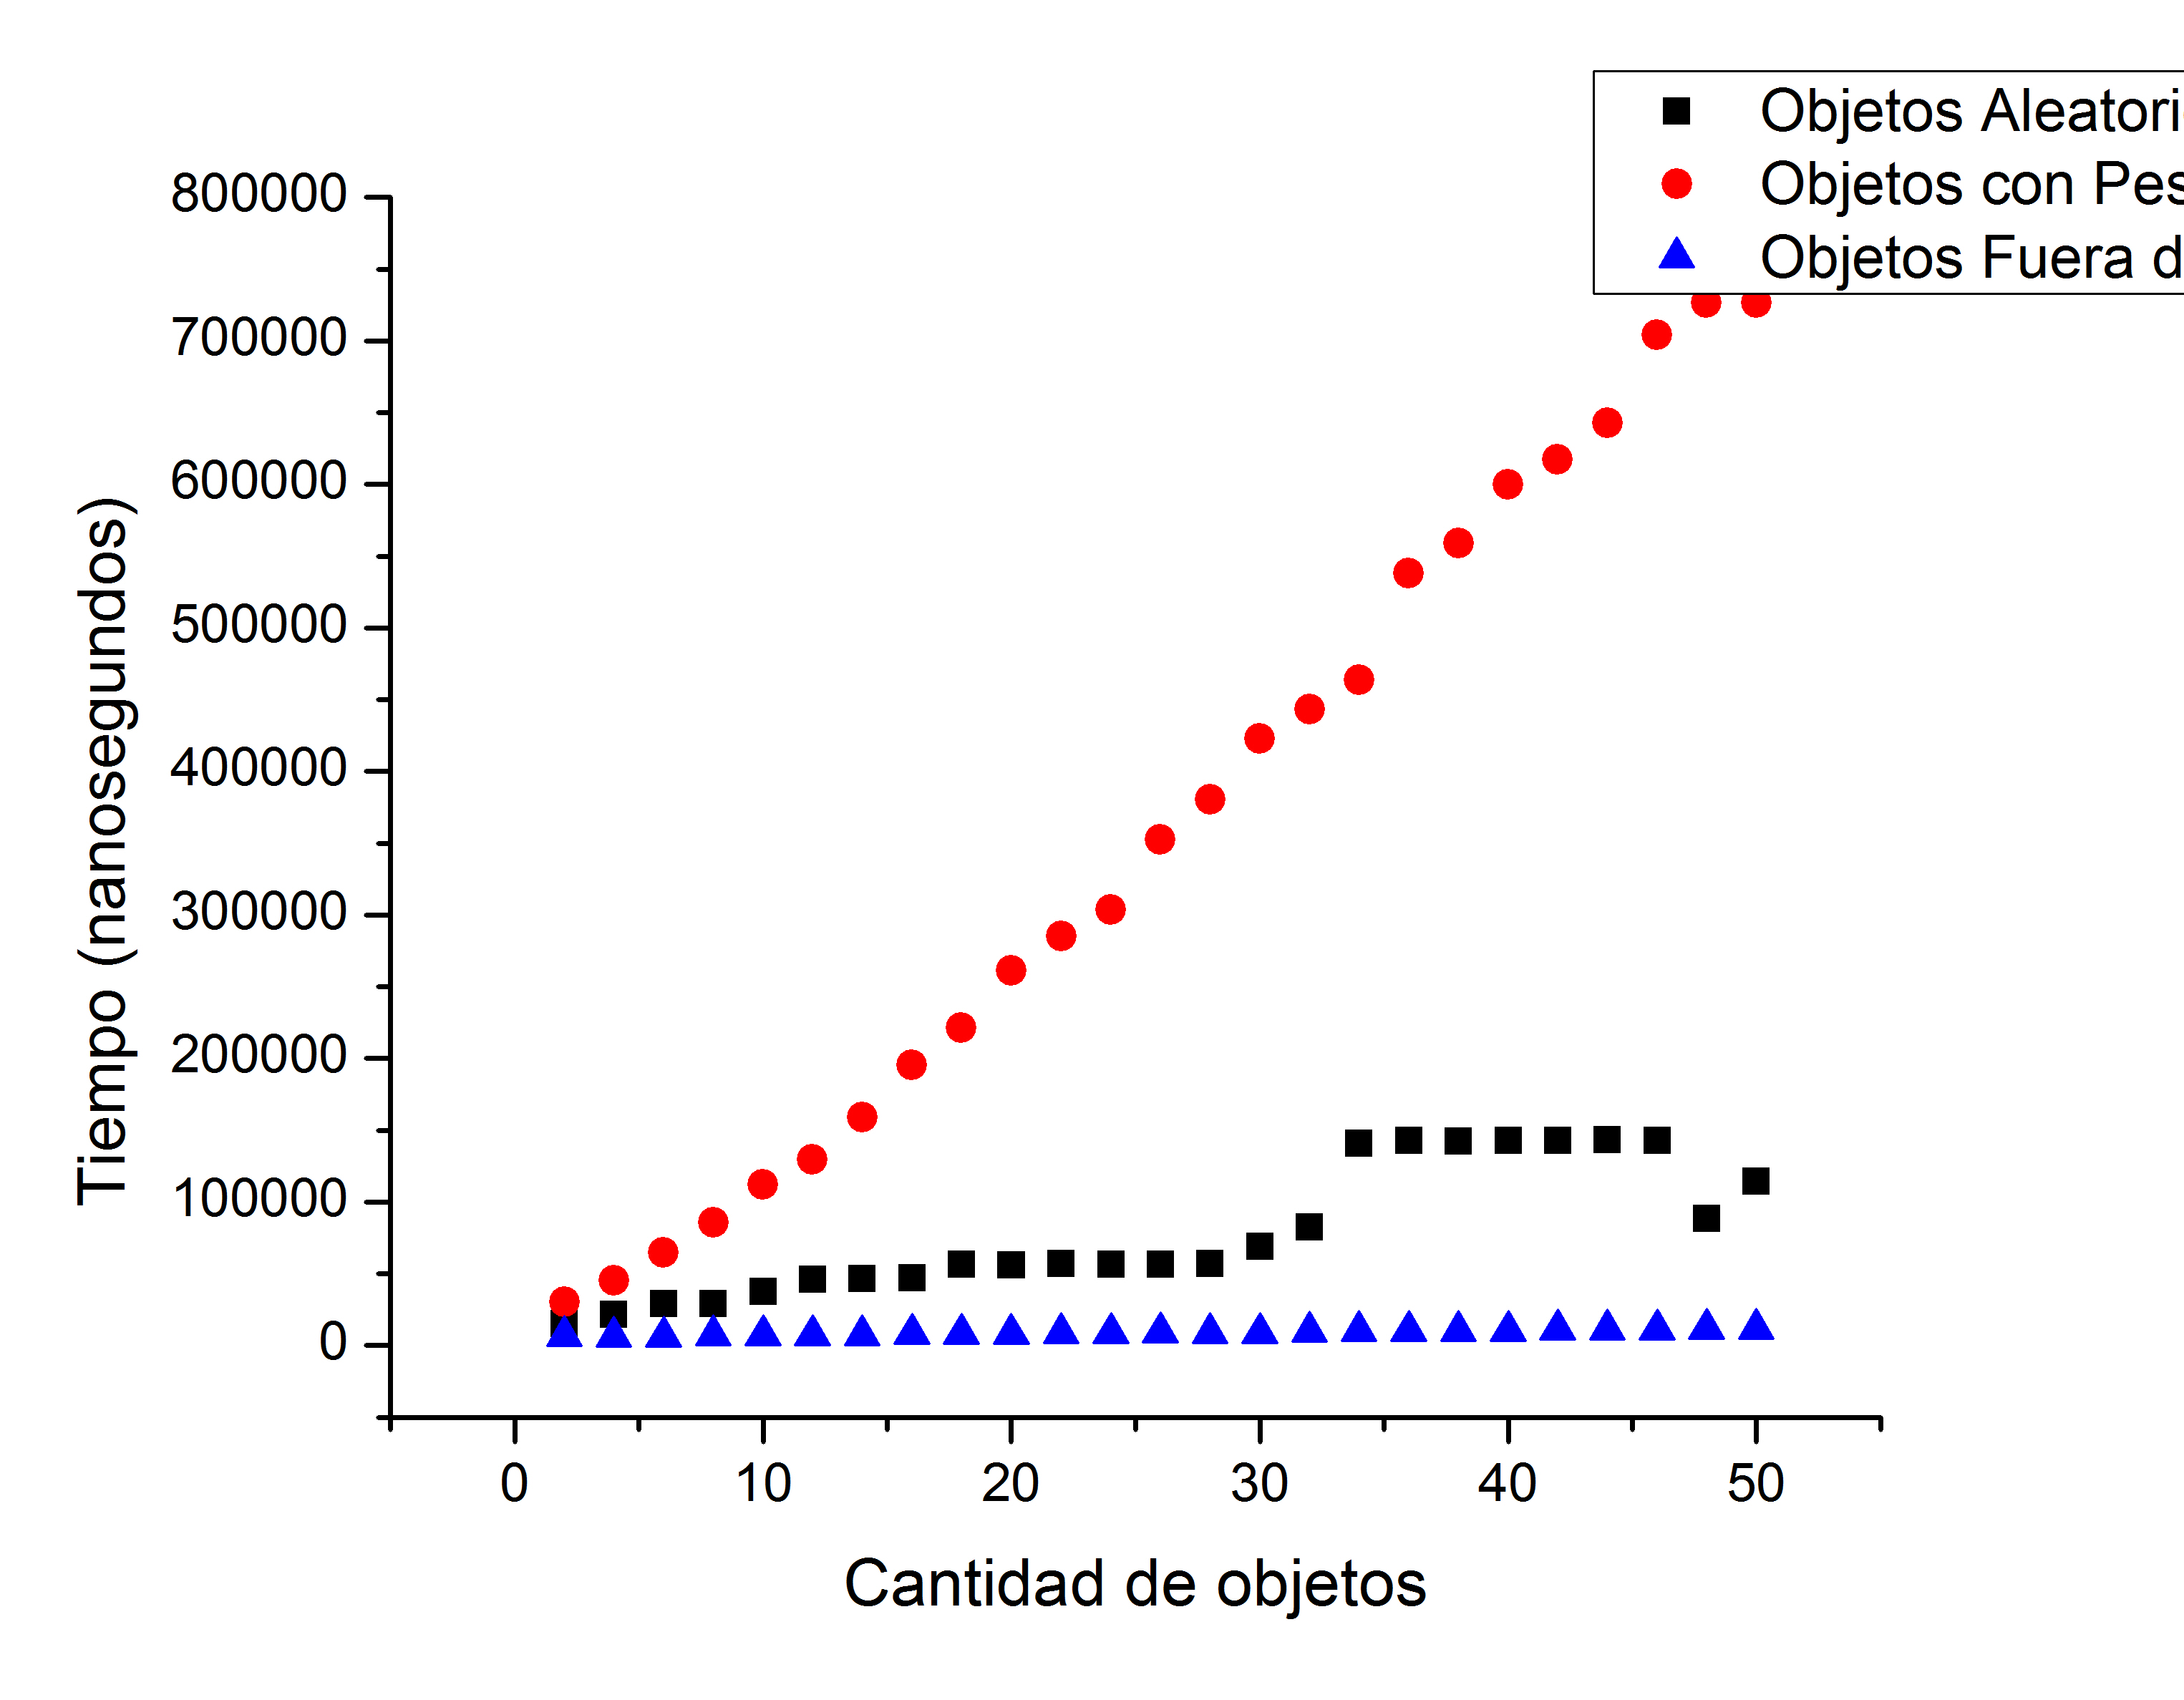
\includegraphics[width=0.4\textwidth]{comparacionObjetos}
\caption{Comparación de los tres casos de nuestro algoritmo variando la cantidad de objetos}
\end{figure}

En esta figura podemos observar no solo la tendencia lineal de la complejidad del algoritmo sino también la variación de las pendientes en cada caso. Notemos que a mayor pendiente, la ejecución toma más tiempo, es decir	 es "más lenta".
En particular podemos destacar que en el caso de que los objetos tengan todos peso mayor a la capacidad de las mochilas, la recta tiende a ser constante. 
  
\begin{figure}[H]
\centering
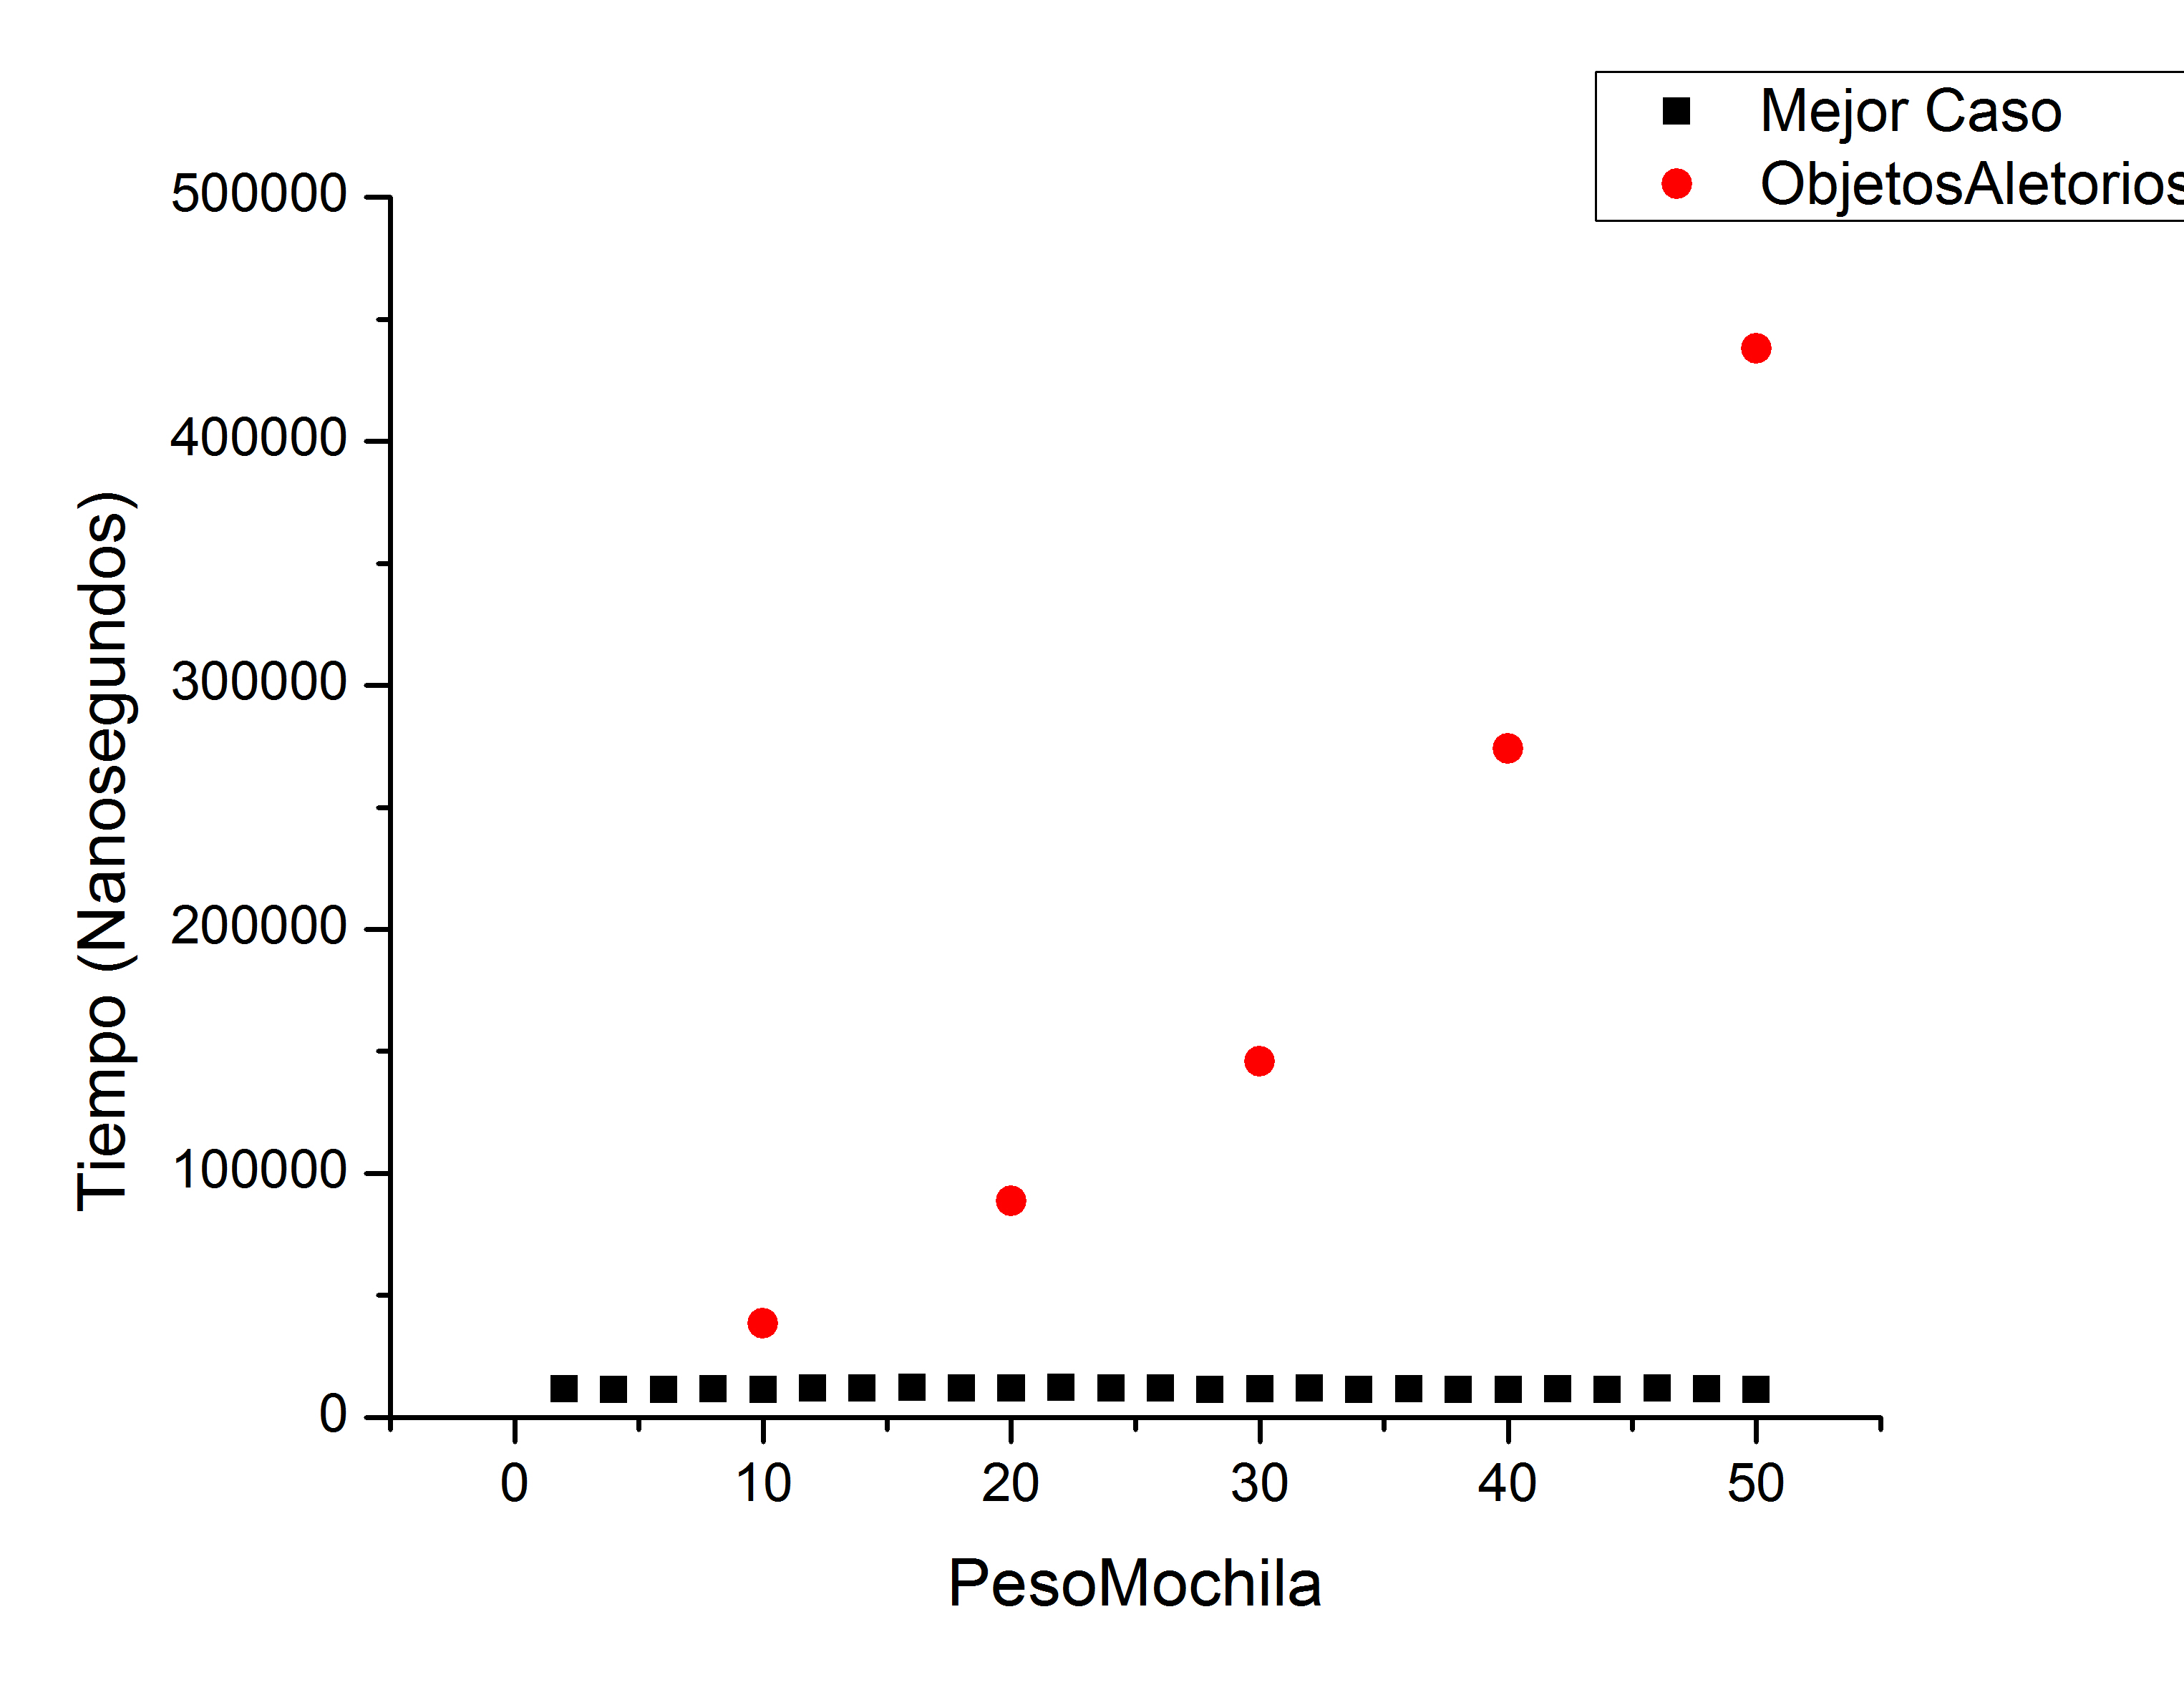
\includegraphics[width=0.4\textwidth]{pesoMCvsObjAl}
\caption{}
\end{figure}

\begin{figure}[H]
\centering
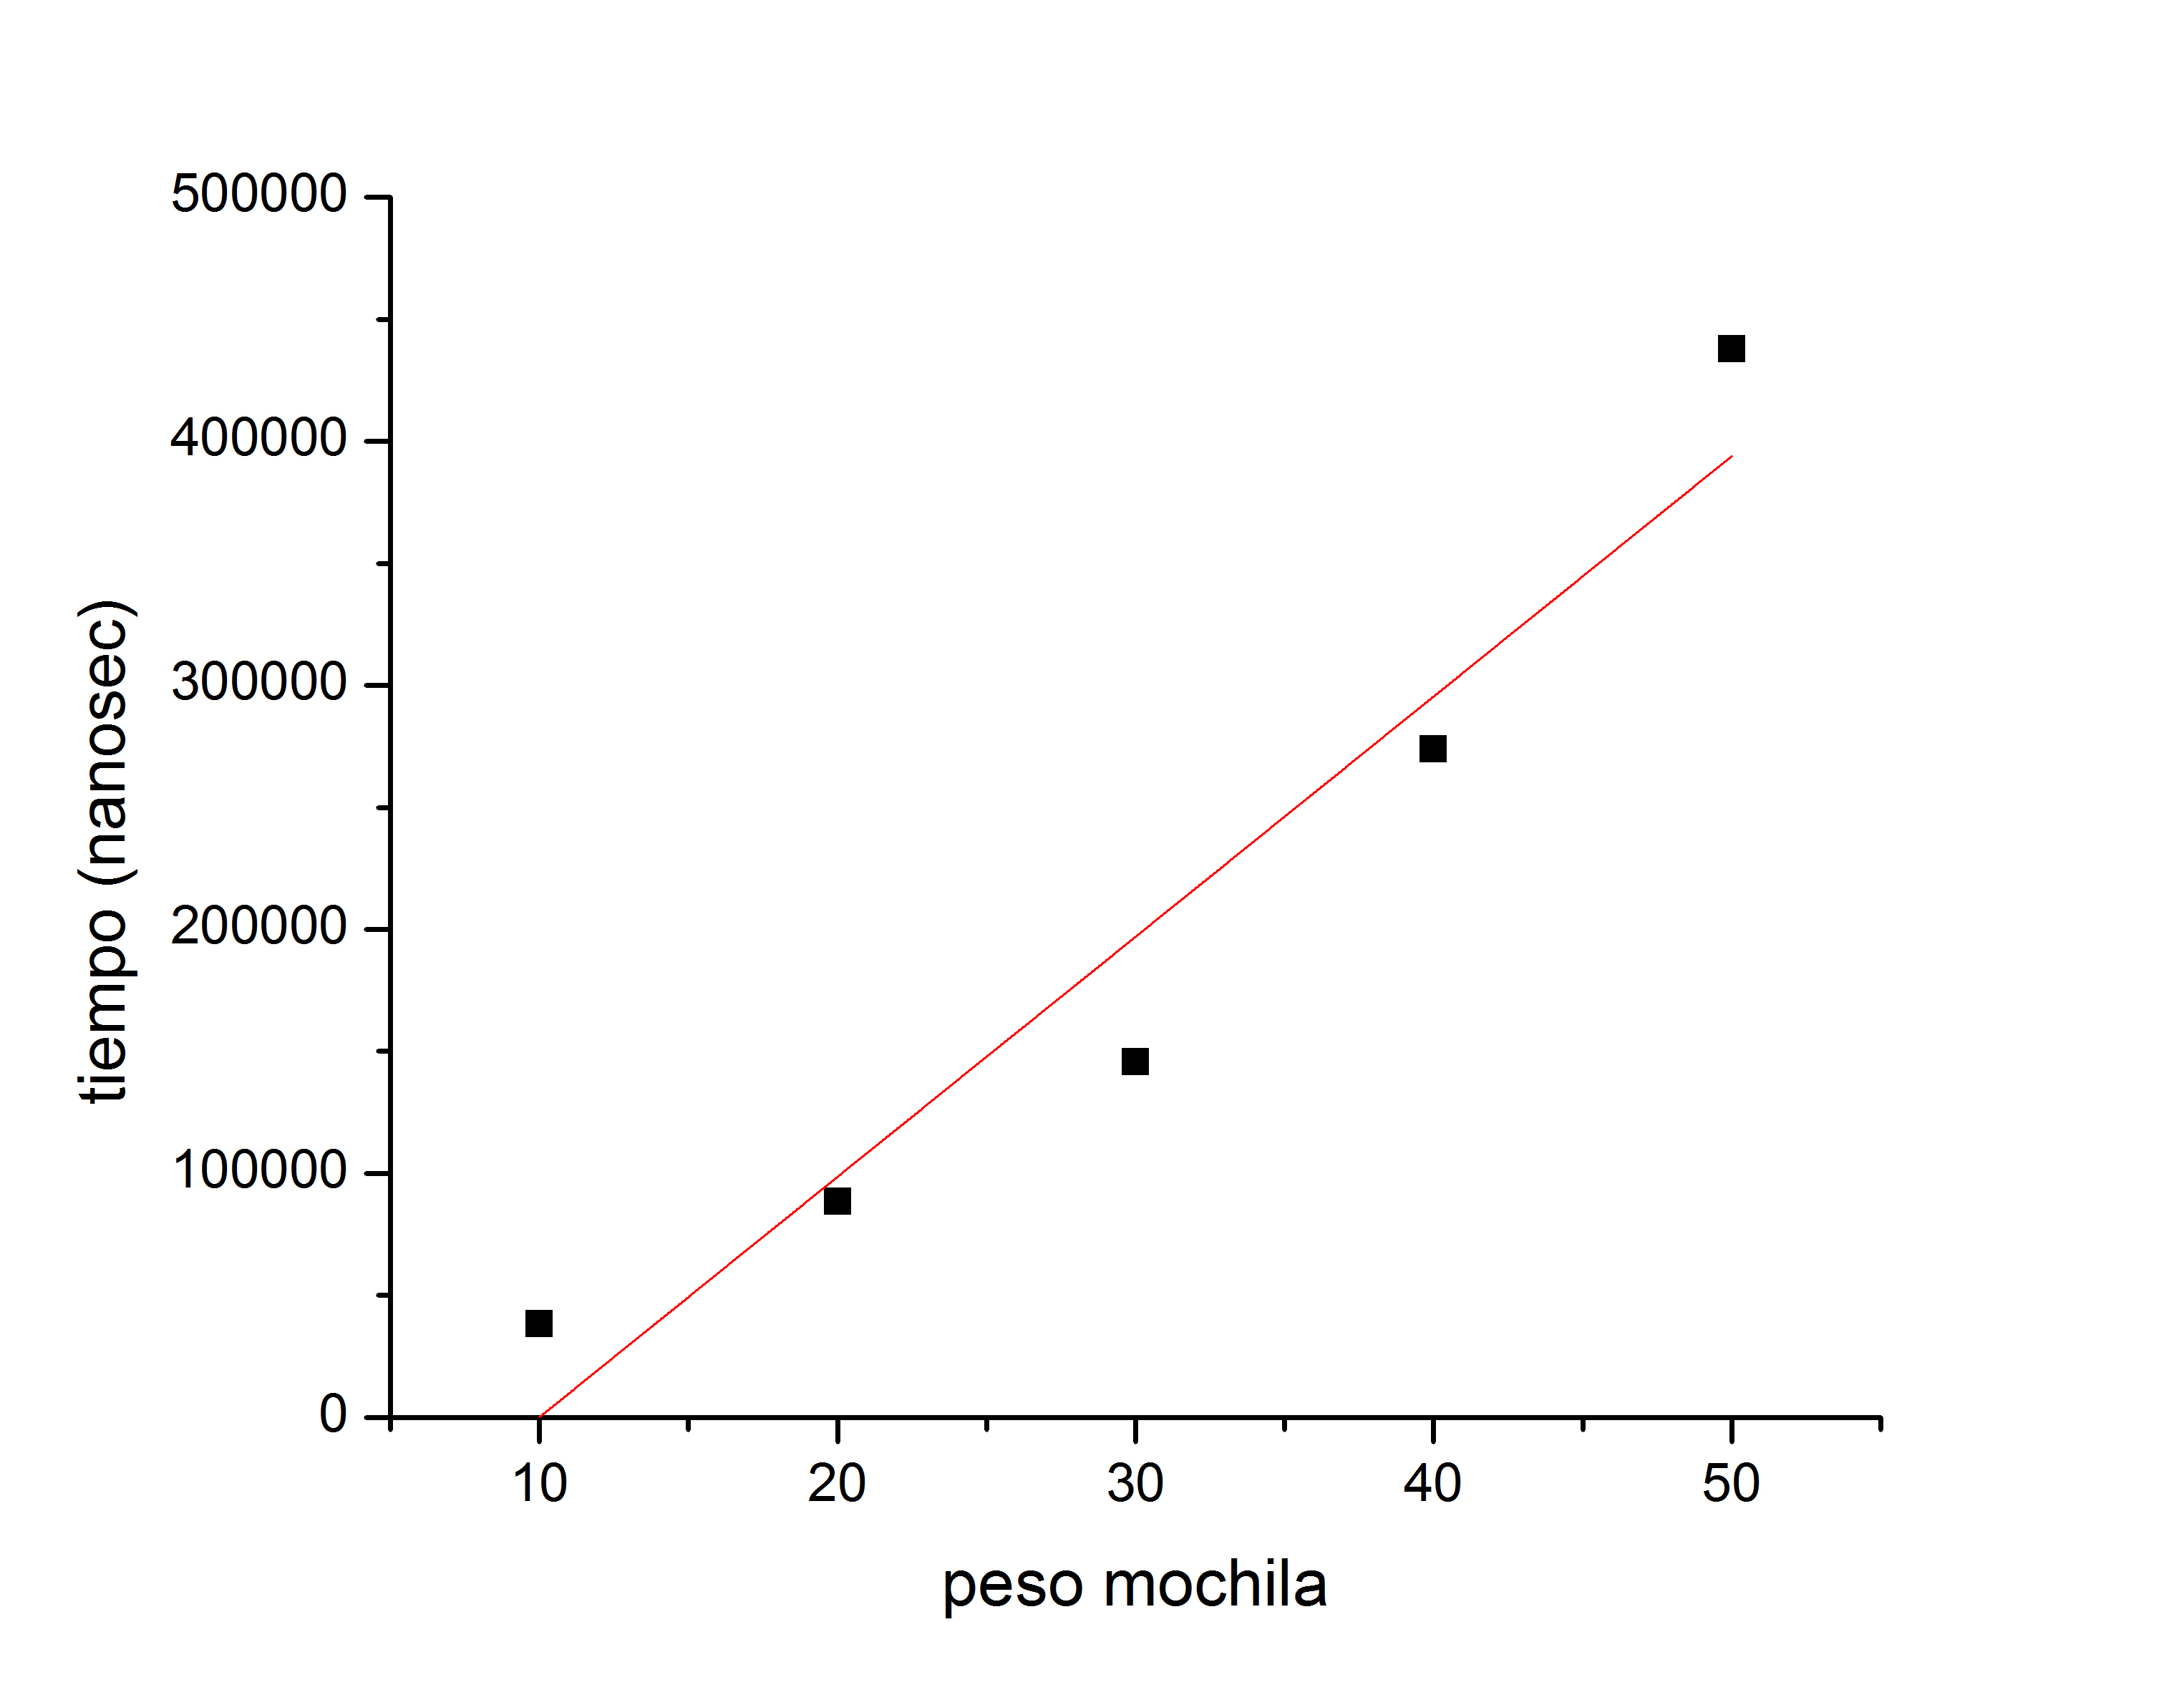
\includegraphics[width=0.4\textwidth]{variacionPesoMoch}
\caption{}
\end{figure}

\subsubsection{Análisis}

\end{document}
